% \documentclass[aspectratio=43]{beamer}

\documentclass[aspectratio=43, handout]{beamer}
% -------------------------------------------------
% Minimal black & white Beamer setup
% -------------------------------------------------

\usepackage{subcaption}

% -------------------------------------------------

\usepackage{fontspec}
\usepackage{unicode-math}

% Serif (opcional)
\setmainfont{Atkinson Hyperlegible}

% Sans (la que usa Beamer)
\setsansfont{Atkinson Hyperlegible}

% Monospace
\setmonofont{Fira Code}

% Matemática
\setmathfont{Latin Modern Math}

\usefonttheme{professionalfonts}

% Hace que beamer use sans como fuente principal
\renewcommand{\familydefault}{\sfdefault}

% Clean black & white appearance
\setbeamercolor{normal text}{fg=black,bg=white}
\setbeamercolor{structure}{fg=black}

% Remove navigation symbols
\setbeamertemplate{navigation symbols}{}
\usefonttheme{professionalfonts} % prevents beamer from overriding fonts

% Simple frame title
\setbeamerfont{frametitle}{series=\bfseries,size=\large}

% Circular bullets (no arrows)
\setbeamertemplate{itemize item}{$\circ$}
\setbeamertemplate{itemize subitem}{$\circ$}
\setbeamertemplate{itemize subsubitem}{$\circ$}

% Optional: remove shadows and gradients
\setbeamertemplate{blocks}[rounded][shadow=false]

% Monospace code setup
\usepackage{listings}

\lstset{
  basicstyle=\ttfamily\small,
  keywordstyle=\bfseries,
  commentstyle=\itshape,
  showstringspaces=false,
  frame=single,
  breaklines=true
}

% -------------------------------------------------
% Title info
% -------------------------------------------------

\title{Óptica geométrica}
\author{Aramayo Martín}
\date{\today}

% -------------------------------------------------
% Document
% -------------------------------------------------

\begin{document}

\begin{frame}
	\titlepage
\end{frame}

% \begin{frame}{Example Bullets}
% 	\begin{itemize}
% 		\item First item
% 		\item Second item
% 		\item Third item
% 	\end{itemize}
% \end{frame}

% \begin{frame}[fragile]{Code Example}

% 	\begin{lstlisting}
% fn main() {
%     println!("Hello, world!");
% }
% \end{lstlisting}

% \end{frame}

\section{Repaso de los tipos de espejo}

\subsection{Repaso de los tipos de espejo: Cómo son los signos}

\begin{frame}{Repaso de los tipos de espejo: Cómo son los signos}
	\qquad

	Por convención, la distancia objeto-espejo $D_o$ es positiva.

	\qquad
	\pause

	Espejo cóncavo

	\pause

	\begin{figure}
		\centering
		
\includegraphics[width=0.6\textwidth]{figurasPDF/concavo-correcto-Signos.pdf}
	\end{figure}

	\pause

	Espejo convexo

	\pause

	\begin{figure}
		\centering
		
\includegraphics[width=0.6\textwidth]{figurasPDF/convexo-correcto-Signos.pdf}
	\end{figure}

\end{frame}

% -------------------------------------------------

\subsection{Repaso de los tipos de espejo: Ecuación de espejos curvos}

\begin{frame}{Repaso de los tipos de espejo: Ecuación de espejos curvos}

	La ecuación de espejos curvos

	\pause

	\begin{figure}
		\centering
		
\includegraphics[width=0.8\textwidth]{figurasPDF/convexo-rayoCuchau.pdf}
	\end{figure}

	\pause

	\[
		\frac{1}{f} = \frac{1}{D_o} + \frac{1}{D_i}
	\]

	\pause

	$D_o$: Distancia del objeto al espejo

	$D_i$: Distancia de la imagen al espejo

	$f$: Distancia focal del espejo ($C=2f=R$)

\end{frame}

% -------------------------------------------------

\subsection{Repaso de los tipos de espejo: Cómo distinguirlos}

\begin{frame}{Repaso de los tipos de espejo: Cómo distinguirlos}

	\pause

	\begin{figure}
		\centering
		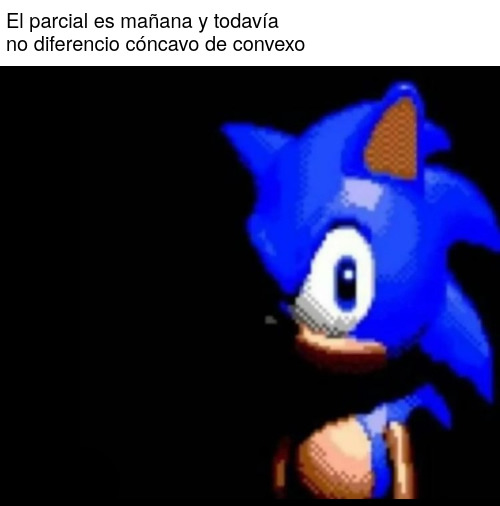
\includegraphics[width=0.766\textwidth]{figurasPDF/sonicTrauma.jpg}

	\end{figure}

\end{frame}

% -------------------------------------------------
\subsection{Repaso de los tipos de espejo: CUCHARA}

\begin{frame}{Repaso de los tipos de espejo: CUCHARA}

	\pause

	\begin{figure}
		\centering
		
\includegraphics[width=0.999\textwidth]{figurasPDF/cucharonPa.pdf}

	\end{figure}

\end{frame}

% -------------------------------------------------

\subsection{Repaso de los tipos de espejo: Espejo Cóncavo}

\begin{frame}{Repaso de los tipos de espejo: Espejo Cóncavo}

	\pause

	Espejo cóncavo

	\pause

	\begin{figure}
		\centering
		\begin{subfigure}{0.355\textwidth}
			\centering
			
\includegraphics[width=\textwidth]{figurasPDF/concavooo-01.pdf}
		\end{subfigure}
		\hfill
		\pause
		\begin{subfigure}{0.355\textwidth}
			\centering
			
\includegraphics[width=\textwidth]{figurasPDF/concavooo-02.pdf}
		\end{subfigure}
	\end{figure}

	\pause

	\begin{figure}
		\centering
		
\includegraphics[width=0.355\textwidth]{figurasPDF/focoConvergenciaPa.jpg}
	\end{figure}

\end{frame}

% -------------------------------------------------

\subsection{Repaso de los tipos de espejo: Espejo Convexo}

\begin{frame}{Repaso de los tipos de espejo: Espejo Convexo}

	Espejo convexo

	\pause

	\begin{figure}
		\centering
		\begin{subfigure}{0.355\textwidth}
			\centering
			
\includegraphics[width=\textwidth]{figurasPDF/convexooo-01.pdf}
		\end{subfigure}
		\pause
		\hfill
		\begin{subfigure}{0.355\textwidth}
			\centering
			
\includegraphics[width=\textwidth]{figurasPDF/convexooo-02.pdf}
		\end{subfigure}
	\end{figure}

	\pause

	\begin{figure}
		\centering
		Maksútov-Cassegrain
		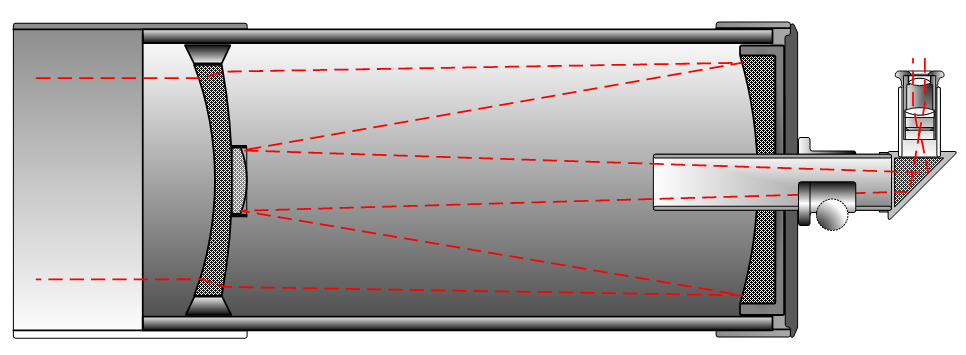
\includegraphics[width=0.8\textwidth]{figurasPDF/Maksutov-Cassegrain.png}
	\end{figure}

\end{frame}

% -------------------------------------------------

\subsection{Repaso de los tipos de espejo: Comparativa de los dos}

\begin{frame}{Repaso de los tipos de espejo: Comparativa de los dos}

	Espejo cóncavo

	\pause
	\begin{figure}
		\centering
		
\includegraphics[width=0.85\textwidth]{figurasPDF/concavooo.pdf}
	\end{figure}

	\pause
	Espejo convexo

	\begin{figure}
		\centering
		
\includegraphics[width=0.85\textwidth]{figurasPDF/convexooo.pdf}
	\end{figure}

\end{frame}

% -------------------------------------------------
% \section{Comparación entre espejo cóncavo y convexo}

% \begin{frame}{Comparación entre espejo cóncavo y convexo}

% 	\small

% 	\begin{tabular}{|p{3.5cm}|p{3.2cm}|p{2.68cm}|}
% 		\hline
% 		\textbf{Característica} & \textbf{Espejo cóncavo} & \textbf{Espejo convexo} \\
% 		\hline
% 		Imágenes                & Reales / virtuales      & Siempre virtuales       \\
% 		\hline
% 		Orientación de imagen   & Invertida / derecha     & Siempre derecha         \\
% 		\hline
% 		Tamaño imagen           & Mayor / menor / igual   & Siempre menor           \\
% 		\hline
% 		Campo visual            & Reducido                & Amplio                  \\
% 		\hline
% 	\end{tabular}

% 	\pause

% 	\quad

% 	% \centerline{\rule{0.9\linewidth}{0.4pt}}\vspace{0.3cm}

% 	\quad

% 	\quad

% 	\quad

% 	\quad

% 	\centering

% 	OJO CON EL CÓNCAVO, MARAVILLA DE LA CREACIÓN

% \end{frame}

% -------------------------------------------------
\section{Diagrama de rayos}

\subsection{Diagrama de rayos: Reglas}
\begin{frame}{Diagrama de rayos: Reglas}

	Podemos usar 3 rayos para ubicar la imagen:

	\pause

	\begin{enumerate}
		\item Un rayo \textbf{paralelo al eje}, después de reflejarse, pasa por el
		      \textbf{punto focal} $F$ de un \textit{espejo cóncavo} o parece provenir del
		      punto focal \textit{(virtual)} de un \textit{espejo convexo}.

		      \pause

		\item Un rayo que pasa por el \textbf{punto focal} $F$
		      (o avanza hacia éste) se refleja \textbf{paralelamente al eje}.

		      \pause

		\item Un rayo a lo largo del radio que pasa por el
		      \textbf{centro de curvatura} $C$, o se acerca a él, intersecta la superficie
		      en dirección normal y se refleja de regreso por su trayectoria original.

		      %       \pause
		      % \item Un rayo que incide en el \textbf{vértice} $V$ se refleja, formando
		      %       ángulos iguales con el \textbf{eje óptico}.
	\end{enumerate}

\end{frame}

% -------------------------------------------------
\subsection{Diagrama de rayos: Reglas resumidas}
\begin{frame}{Diagrama de rayos: Reglas resumidas}

	Resumen:
	\pause
	\begin{enumerate}
		\item \textbf{Paralelo al eje} $\rightarrow$ \textbf{Foco}

		      \pause

		\item \textbf{Foco} $\rightarrow$ \textbf{Paralelo al eje}

		      \pause

		\item \textbf{Centro} $\rightarrow$ \textbf{Centro} (Se refleja sobre sí mismo)

		      %       \pause
		      % \item Un rayo que incide en el \textbf{vértice} $V$ se refleja, formando
		      %       ángulos iguales con el \textbf{eje óptico}.
	\end{enumerate}

\end{frame}

% -------------------------------------------------

\section{Diagrama de rayos: Ejemplos}

% -------------------------------------------------

\subsection{Diagrama de rayos: Espejo Convexo}

\begin{frame}{Diagrama de rayos: Espejo Convexo}

	Las reglas aplican al espejo convexo:

	\begin{figure}
		\centering
		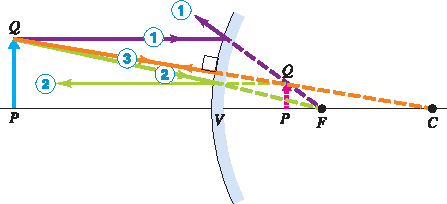
\includegraphics[width=0.8\textwidth]{figurasPDF/convexo-full.pdf}
	\end{figure}

	\vfill
	\vfill
	\vfill
	\vfill
\end{frame}
\subsection{Diagrama de rayos: Espejo Convexo, Rayo 1}
\begin{frame}{Diagrama de rayos: Espejo Convexo, Rayo 1}

	Las reglas aplican al espejo convexo:

	\begin{figure}
		\centering
		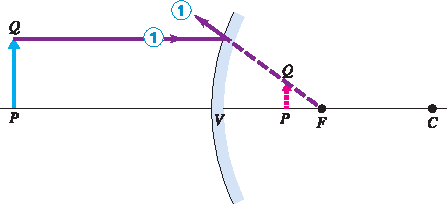
\includegraphics[width=0.8\textwidth]{figurasPDF/convexo-rayo01.pdf}
	\end{figure}

	\pause
	1. Un rayo \textbf{paralelo al eje}, después de reflejarse, pasa por el
	\textbf{punto focal} $F$ de un \textit{espejo cóncavo} o parece provenir del
	punto focal \textit{(virtual)} de un \textit{espejo convexo}.

	\pause
	\centerline{\rule{0.9\linewidth}{0.4pt}}\vspace{0.3cm}

	1. \textbf{Paralelo al eje} $\rightarrow$ \textbf{Foco}

\end{frame}

% -------------------------------------------------

\subsection{Diagrama de rayos: Espejo Convexo, Rayo 2}
\begin{frame}{Diagrama de rayos: Espejo Convexo, Rayo 2}

	Las reglas aplican al espejo convexo:

	\begin{figure}
		\centering
		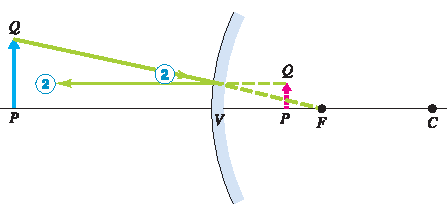
\includegraphics[width=0.8\textwidth]{figurasPDF/convexo-rayo02.pdf}
	\end{figure}

	\pause
	2. Un rayo que pasa por el \textbf{punto focal} $F$
	(o avanza hacia éste) se refleja \textbf{paralelamente al eje}.

	\pause
	\centerline{\rule{0.9\linewidth}{0.4pt}}\vspace{0.3cm}

	2. \textbf{Foco} $\rightarrow$ \textbf{Paralelo al eje}

\end{frame}

% -------------------------------------------------
\subsection{Diagrama de rayos: Espejo Convexo, Rayo 3}
\begin{frame}{Diagrama de rayos: Espejo Convexo, Rayo 3}

	Las reglas aplican al espejo convexo:

	\begin{figure}
		\centering
		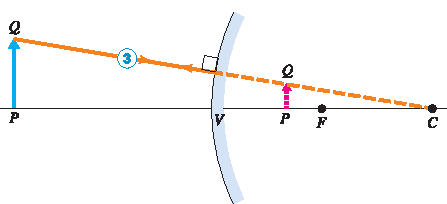
\includegraphics[width=0.8\textwidth]{figurasPDF/convexo-rayo03.pdf}
	\end{figure}

	\pause
	3. Un rayo a lo largo del radio que pasa por el
	\textbf{centro de curvatura} $C$, o se acerca a él, intersecta la superficie
	en dirección normal y se refleja de regreso por su trayectoria original.

	\pause
	\centerline{\rule{0.9\linewidth}{0.4pt}}\vspace{0.3cm}

	3. \textbf{Centro} $\rightarrow$ \textbf{Centro} (Se refleja sobre sí mismo)

\end{frame}

% -------------------------------------------------

\subsection{Diagrama de rayos: Espejo Cóncavo}

\begin{frame}{Diagrama de rayos: Espejo Cóncavo}

	Las reglas aplicadas al espejo cóncavo

	\pause

	\begin{figure}
		\centering
		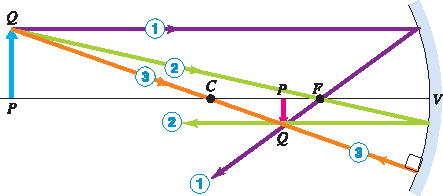
\includegraphics[width=0.8\textwidth]{figurasPDF/concavo-full.pdf}
	\end{figure}

	\vfill
	\vfill
	\vfill
	\vfill
\end{frame}

% -------------------------------------------------

\subsection{Diagrama de rayos: Espejo Cóncavo, Rayo 1}

\begin{frame}{Diagrama de rayos: Espejo Cóncavo, Rayo 1}

	Las reglas aplicadas al espejo cóncavo

	\begin{figure}
		\centering
		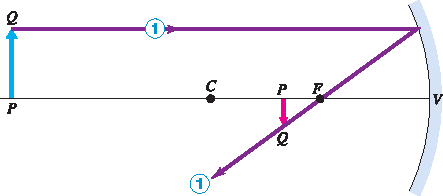
\includegraphics[width=0.8\textwidth]{figurasPDF/concavo-rayo01.pdf}
	\end{figure}

	\pause

	1. Un rayo \textbf{paralelo al eje}, después de reflejarse, pasa por el
	\textbf{punto focal} $F$ de un \textit{espejo cóncavo} o parece provenir del
	punto focal \textit{(virtual)} de un \textit{espejo convexo}.

	\pause

	\centerline{\rule{0.9\linewidth}{0.4pt}}\vspace{0.3cm}

	1. \textbf{Paralelo al eje} $\rightarrow$ \textbf{Foco}
\end{frame}

% -------------------------------------------------

\subsection{Diagrama de rayos: Espejo Cóncavo, Rayo 2}

\begin{frame}{Diagrama de rayos: Espejo Cóncavo, Rayo 2}

	Las reglas aplicadas al espejo cóncavo:

	\begin{figure}
		\centering
		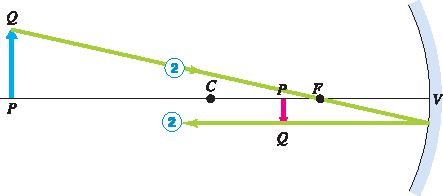
\includegraphics[width=0.8\textwidth]{figurasPDF/concavo-rayo02.pdf}
	\end{figure}

	\pause

	2. Un rayo que pasa por el \textbf{punto focal} $F$
	(o avanza hacia éste) se refleja \textbf{paralelamente al eje}.

	\pause

	\centerline{\rule{0.9\linewidth}{0.4pt}}\vspace{0.3cm}

	2. \textbf{Foco} $\rightarrow$ \textbf{Paralelo al eje}

\end{frame}

% -------------------------------------------------

\subsection{Diagrama de rayos: Espejo Cóncavo, Rayo 3}

\begin{frame}{Diagrama de rayos: Espejo Cóncavo, Rayo 3}

	Las reglas aplicadas al espejo cóncavo:

	\begin{figure}
		\centering
		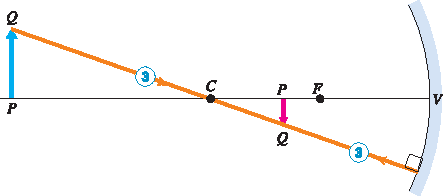
\includegraphics[width=0.8\textwidth]{figurasPDF/concavo-rayo03.pdf}
	\end{figure}

	\pause

	3. Un rayo a lo largo del radio que pasa por el
	\textbf{centro de curvatura} $C$, o se acerca a él, intersecta la superficie
	en dirección normal y se refleja de regreso por su trayectoria original.

	\pause

	\centerline{\rule{0.9\linewidth}{0.4pt}}\vspace{0.3cm}

	3. \textbf{Centro} $\rightarrow$ \textbf{Centro} (Se refleja sobre sí mismo)

\end{frame}

% -------------------------------------------------
\section{El espejo cóncavo...}
\begin{frame}{El espejo cóncavo...}

	\begin{figure}
		\centering
		
\includegraphics[width=0.67\textwidth]{figurasPDF/sonicCONCAVO.jpg}

	\end{figure}

\end{frame}
% -------------------------------------------------

\section{El espejo cóncavo es especial}

% -------------------------------------------------

\subsection{El espejo cóncavo es especial: Objeto entre el vertice y el foco}

\begin{frame}{El espejo cóncavo es especial: Objeto entre el vertice y el foco}

	Distancia de objeto entre el foco y el vértice

	$$0 < D_o < F$$

	\pause

	\quad

	\begin{figure}
		\centering
		
\includegraphics[width=0.7\textwidth]{figurasPDF/concavoDificil04.pdf}
	\end{figure}

\end{frame}

% -------------------------------------------------

\subsection{El espejo cóncavo es especial: Objeto en el foco}

\begin{frame}{El espejo cóncavo es especial: Objeto en el foco}

	Distancia de objeto igual a la distancia al foco

	$$D_o = F$$

	\pause

	\quad

	\begin{figure}
		\centering
		
\includegraphics[width=0.7\textwidth]{figurasPDF/concavoDificil03.pdf}
	\end{figure}

\end{frame}

% -------------------------------------------------

\subsection{El espejo cóncavo es especial: Objeto entre el centro y el foco}

\begin{frame}{El espejo cóncavo es especial: Objeto entre el centro y el foco}

	Distancia de objeto, entre el centro y el foco

	$$F < D_o < C$$

	\pause

	\quad

	\begin{figure}
		\centering
		
\includegraphics[width=0.7\textwidth]{figurasPDF/concavoDificil05.pdf}
	\end{figure}

\end{frame}

% -------------------------------------------------

\subsection{El espejo cóncavo es especial: Objeto en el centro}

\begin{frame}{El espejo cóncavo es especial: Objeto en el centro}

	Distancia de objeto igual a la distancia al centro

	$$D_o = C$$

	\pause

	\quad

	\begin{figure}
		\centering
		
\includegraphics[width=0.7\textwidth]{figurasPDF/concavoDificil02.pdf}
	\end{figure}

\end{frame}

% -------------------------------------------------

\subsection{El espejo cóncavo es especial: Objeto más allá del centro}

\begin{frame}{El espejo cóncavo es especial: Objeto más allá del centro}

	Distancia de objeto mayor a la distancia del centro

	$$C < D_o$$

	\pause

	\begin{figure}
		\centering
		
\includegraphics[width=0.7\textwidth]{figurasPDF/concavoDificil01.pdf}
	\end{figure}

\end{frame}

% -------------------------------------------------

\subsection{El espejo cóncavo es especial: Je todos juntos}

\begin{frame}{El espejo cóncavo es especial: Je todos juntos}

	\scriptsize

	\begin{figure}
		\centering

		% Primera fila
		\begin{minipage}{0.32\textwidth}
			\centering
			Objeto entre foco y vértice\\[0.2em]
			
\includegraphics[width=\linewidth]{figurasPDF/concavoDificil04.pdf}
		\end{minipage}
		\
		\begin{minipage}{0.32\textwidth}
			\centering
			Objeto entre el foco y el centro\\[0.2em]
			
\includegraphics[width=\linewidth]{figurasPDF/concavoDificil05.pdf}
		\end{minipage}
		\
		\begin{minipage}{0.32\textwidth}
			\centering
			Objeto más allá del centro\\[0.2em]
			
\includegraphics[width=\linewidth]{figurasPDF/concavoDificil01.pdf}
		\end{minipage}
		\vspace{1.5em}

		% Segunda fila
		\begin{minipage}{0.32\textwidth}
			\centering
			Objeto en el centro\\[0.2em]
			
\includegraphics[width=\linewidth]{figurasPDF/concavoDificil02.pdf}
		\end{minipage}
		\qquad
		\begin{minipage}{0.32\textwidth}
			\centering
			Objeto en el foco\\[0.2em]
			
\includegraphics[width=\linewidth]{figurasPDF/concavoDificil03.pdf}
		\end{minipage}

	\end{figure}

\end{frame}
% -------------------------------------------------
% \section{Espejo cóncavo, TODOS LOS ESTILOS}
% \begin{frame}{Espejo cóncavo, TODOS LOS ESTILOS}

% 	Posición del objeto

% 	\quad

% 	\begin{tabular}{|p{2.3cm}|p{3.15cm}|p{4.65cm}|}
% 		\hline
% 		{\boldmath $\boldmath \mathbf{D_o}$} & \textbf{Objeto}            & \textbf{Imagen} \\
% 		\hline

% 		\centering$0 < D_o < F$
% 		                                     & Entre espejo y foco
% 		                                     & Virtual, derecha aumentada                   \\
% 		\hline

% 		$F = D_o$ \hfill
% 		                                     & En el foco
% 		                                     & En $\infty$                                  \\
% 		\hline

% 		\centering$F < D_o < C$
% 		                                     & Entre foco y centro
% 		                                     & Real, invertida, aumentada                   \\
% 		\hline

% 		\hfill $D_o = C$ \hfill
% 		                                     & En el centro
% 		                                     & Real, invertida, igual                       \\
% 		\hline

% 		$C < D_o$
% 		                                     & Más allá del centro
% 		                                     & Real, invertida, reducida                    \\
% 		\hline

% 	\end{tabular}

% \end{frame}

% -------------------------------------------------
\section{Espejos, TODOS LOS ESTILOS}
\begin{frame}{Espejos, TODOS LOS ESTILOS}

	\pause

	Espejo cóncavo, Cómo queda la imagen según el valor de $D_o$

	\begin{figure}
		\centering
		
\includegraphics[width=0.95\textwidth]{figurasPDF/espejoConcavo-fases.pdf}
	\end{figure}

	\pause

	Espejo convexo, Cómo queda la imagen según el valor de $D_o$
	\begin{figure}
		\centering
		
\includegraphics[width=0.95\textwidth]{figurasPDF/espejoConvexo-fases.pdf}
	\end{figure}

\end{frame}

% -------------------------------------------------
\begin{frame}

	Eso es todo

	\begin{figure}
		\centering
		
\includegraphics[width=0.7\textwidth]{figurasPDF/listoBe.jpg}
	\end{figure}

\end{frame}

\end{document}
